\documentclass[11pt]{beamer}
\usepackage[utf8]{inputenc}
\usepackage[T1]{fontenc}
\usepackage{lmodern}
\usepackage[spanish,english]{babel}
\usetheme{metropolis}
\usepackage{graphicx}
\usepackage{listings}
\begin{document}
    \author{UTIM}
    \title{Notas}
    %\subtitle{}
    %\logo{}
    %\institute{}
    %\date{}
    %\subject{}
    %\setbeamercovered{transparent}
    %\setbeamertemplate{navigation symbols}{}
    \begin{frame}[plain]
        \maketitle
    \end{frame}


    \section{Columnas, columnas guardianes su utilidad y cuidados}
      \subsection{Columnas guardianes}

      \begin{frame}{Columnas guardianes}
          \begin{itemize}
              \item Para darle larga vida a la columna, use siempre la columna guardián. La columna guardián \textbf{previene posibles obstrucciones en la columna} producto de un mal filtrado o algún precipitado que se forme antes de la misma.
              \item La columna guardián es la composicion del cartucho más el holder (sostén o lo que agarra al cartucho).
              \item En este laboratorio (UTIM) contamos con la columna de Phenomenex Parts No: AJ0-9000(Cartucho) y AJ0-9000(Holder).
          \end{itemize}

      \end{frame}
      \begin{frame}{Columnas guardianes. Esquema.}
          \begin{figure}
              \centering
              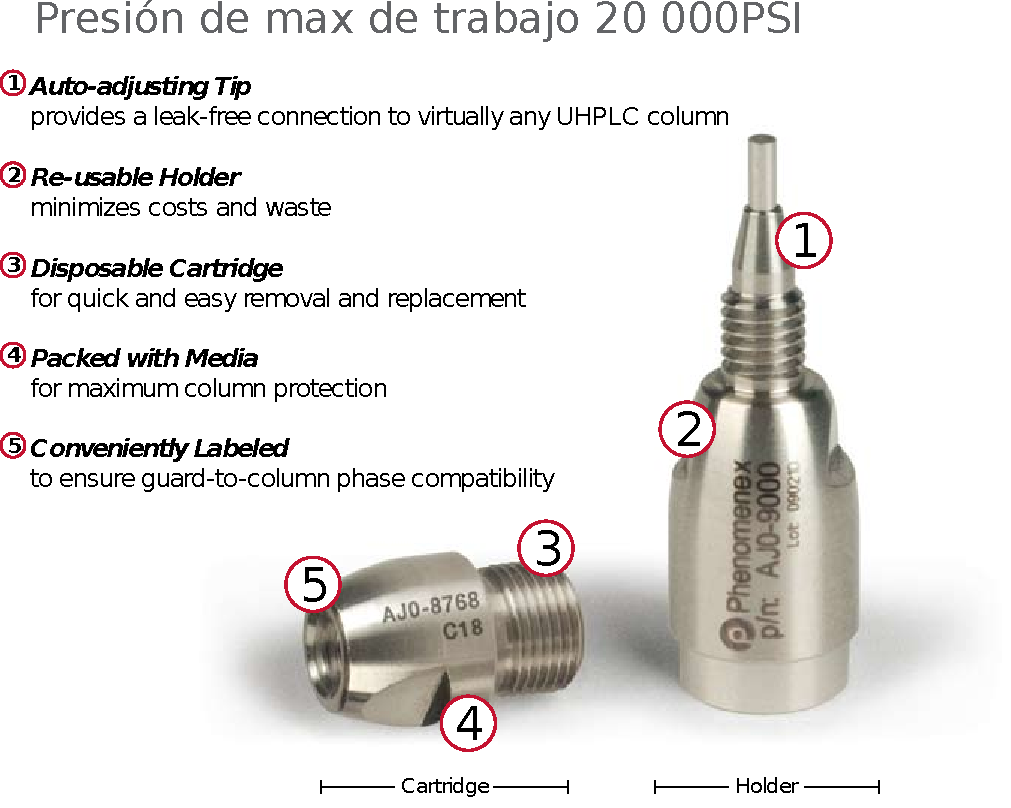
\includegraphics[width=0.9\linewidth]{img/drawing_1}
              \label{fig:drawing1}
          \end{figure}
      \end{frame}
      \begin{frame}{Columnas guardianes. Esquema.}
          \begin{figure}
              \centering
              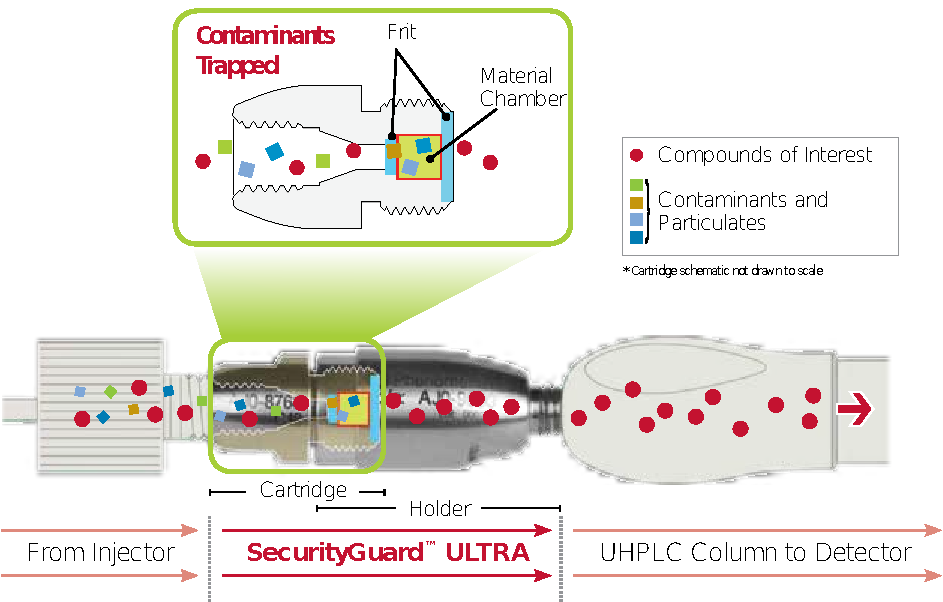
\includegraphics[width=1.0\linewidth]{img/drawing_2}
              \label{fig:drawing2}
          \end{figure}
      \end{frame}

      \subsection{Sobre las columnas nuevas}

      \begin{frame}{Buenas practicas (Columnas)}
        Según WATERS(el fabricante de todas las columnas que hoy tenemos), antes de darle uso a cualquier columna proporcionada por ellos se deben hacer dos procedimientos.
        \begin{enumerate}
            \item Condicionar la columna con fase orgánica. Pasar exclusivamente \textbf{ACETONITRILO}.
            \item Cada columna viene con una ficha técnica o certificado de calidad  emitido por el fabricante. Bajo similares condiciones se debe probar la columna para verificar la integridad de la misma.
        \end{enumerate}
       NOTA: En caso que el certificado técnico no venga en la caja, se puede buscar en la siguiente liga:
       \href{https://support.waters.com/KB_Chem/Columns/WKB10151_How_to_obtain_a_copy_of_Certificate_of_Analysis_CoA_and_Efficiency_Test_Report_for_Waters_Columns_or_Sample_Kits}{Información de la columna. \textbf{click aquí}.}
      \end{frame}
      \begin{frame}{Links}
         https://support.waters.com/KB\_Chem/Columns/WKB10151\_How\_to\_obtain\_a\_copy\_of\_Certificate\_of\_Analysis\_CoA\_and\_Efficiency\_Test\_Report\_for\_Waters\_Columns\_or\_Sample\_Kits
      \end{frame}




    \section{Lavado de columnas Acquity Hibridas de la compañía  Waters }
      \begin{frame}{Lavado de columnas Acquity Hibridas de la compañía  Waters}
        \begin{block}{PROCEDIMIENTO:}
            \begin{enumerate}
                \item Purgar las líneas de la bomba al 100\% de solvente con la siguiente secuencia, línea \textbf{ A} (Agua), \textbf{B} (Acetonitrilo), \textbf{C} (Tetrahidrofurano).
                \item Verificar que no existan tuberías de \textbf{peek} conectadas en el sistema Acquity UPLC.
                \item Antes de iniciar el proceso de lavado de la columna debe de asegurarse que el solvente en su columna es miscible con el solvente recomendado para dicha limpieza.
                \item La velocidad de flujo debe ser de una quinta parte a un medio de la velocidad de flujo normal.

            \end{enumerate}
        \end{block}
      \end{frame}
      \begin{frame}{Lavado de columnas Acquity Hibridas de la compañía  Waters}
          \begin{block}{PROCEDIMIENTO:}
              \begin{enumerate}
                  \item[5.] Estimar el volumen de columna usando la siguiente ecuación: $V=\pi r^2 L$, L representa la longitud y r el radio de la columna respectivamente.
                  \item[6.] Conectar la columna al equipo UPLC e ingresar al link de usos y cuidados que viene indicada en cada una de las columnas híbridas al ser conectado el chip en el horno de columnas de los equipos Acquity.
              \end{enumerate}
          \end{block}
      \end{frame}
      \begin{frame}{Lavado de columnas Acquity Hibridas de la compañía  Waters}
          \begin{block}{PROCEDIMIENTO:}
              \begin{enumerate}

                  \item[7.] Realizar el lavado con 10 volúmenes de columna en el siguiente orden para columnas de fase reversa:
                  \begin{itemize}
                      \item 95\% de agua grado HPLC y 5\% de Acetonitrilo (con la finalidad de remover buffer).
                      \item 100\% de THF grado HPLC.
                      \item 95\% de Acetonitrilo grado HPLC y 5\% de agua grado HPLC.
                      \item Guardarse en 100\% Acetonitrilo grado HPLC.
                  \end{itemize}

              \end{enumerate}
          \end{block}
      \end{frame}
    \section{Limpieza Preventiva y de Mantenimiento}
      \begin{frame}{Fases para la limpieza}
          \textbf{{\Large }SIEMPRE HACER ESTE PROCEDIMIENTO SIN COLUMNA}
          \begin{table}[!h]
              \centering
              \caption{Tabla de solventes}
              \label{tab:tablasolvente}
              \begin{tabular}{c|c}
                  Solvente: Ácido & Solvente: Orgánica \\
                  \hline
                  A = 10\%: B = 90\%  & A = 20\%: B = 40\%: C = 40\%  \\
                  \hline
                  A = $H_2O$    & A = $H_2O$  \\
                  B = $H_2PO_4$ & B = $Isopropilico$  \\
                  & C = $Acetonitrilo$ \\
                  \hline
              \end{tabular}
          \end{table}

          \textbf{{\Large }SIEMPRE HACER ESTE PROCEDIMIENTO SIN COLUMNA}
      \end{frame}
    \section{Limpieza Preventiva}


      \begin{frame}{Limpieza Preventiva}
         \textbf{{\Large }SIEMPRE HACER ESTE PROCEDIMIENTO SIN COLUMNA}

         Las limpiezas tanto preventivas como de mantenimiento se hacen para prevenir la formación y crecimiento de materia biológica o la aparición de sarro en la lineas del equipo.
         \begin{block}{¿Cuando hacer la limpieza preventiva y a cual linea?}
             La limpieza preventiva se debe realizar\textbf{ una vez por semana o cada dos semanas} según las condiciones del laboratorio: hermeticidad, humedad, temperatura etc.

             Esta, solo se realiza a la linea que lleva $H_2O$ y de le debe pasar la fase orgánica de la Tabla:\ref{tab:tablasolvente}.
             Condiciones: \textbf{Flujo de 1mL/min} durante \textbf{30min}.
         \end{block}
         \textbf{{\Large }SIEMPRE HACER ESTE PROCEDIMIENTO SIN COLUMNA}
      \end{frame}

    \section{Limpieza Mantenimiento}
      \begin{frame}{Limpieza de Mantenimiento}
        \textbf{{\Large }SIEMPRE HACER ESTE PROCEDIMIENTO SIN COLUMNA}

        \begin{block}{¿Cuando hacer el mantenimiento y a cual linea?}
          El mantenimiento se debe realizar \textbf{una vez 3 meses} o cuando el sistema este sucio.

          Con un \textbf{flujo 1mL/min},   Pasar 25\% Realizar \textbf{10 inyección con 3 viales}.
          \begin{itemize}
              \item $H_2O$ (25)
              \item Ácido (25)
              \item Orgánico (25)
          \end{itemize}

       \end{block}

       \textbf{{\Large }SIEMPRE HACER ESTE PROCEDIMIENTO SIN COLUMNA}
      \end{frame}
    \section{Cuidados del equipo HPLC AquityArc}
      \begin{frame}{Fin de semana y cuando no se use por mas de dos días consecutivos}
          Se debe/n poner las lineas de agua en fase 10:90 (V:V) acetonitrilo:agua.
      \end{frame}

    \section{Documentación}
      \begin{frame}{Documentación}

        \href{https://www.manualsdir.com/brands/waters/129.html}{Manuales}

        \href{https://www.waters.com/waters/support.htm?locale=es\_EC\&lid=134658708\&cid=511442\&type=USRM}{Otro Manual}


      \end{frame}
    \section{Aplicaciones}
      \begin{frame}{Generalidades}
          La diferencia a tener en cuenta entre los modelos XBridge, XSelect y Cortecs radica fundamentalmente en el tipo de partícula empleada en el empaquetado de la columna. El residuo orgánico que es la cadena que favorece la separación puede estar presente en cada tipo de columna.
          \begin{figure}
              \centering
              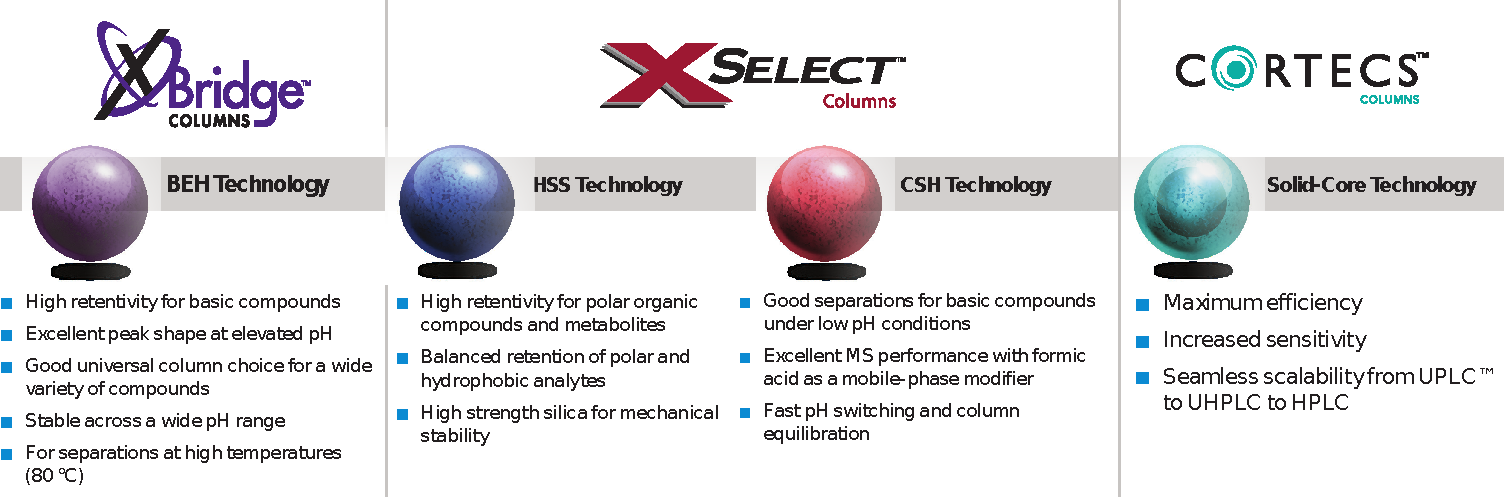
\includegraphics[width=1\linewidth]{img/drawing_3}
              \label{fig:drawing3}
          \end{figure}
      \end{frame}



      \subsection{CORTECS}
        \begin{frame}{}
            \begin{center}
                \textbf{\LARGE Cortecs}
            \end{center}
            \begin{figure}
                \centering
                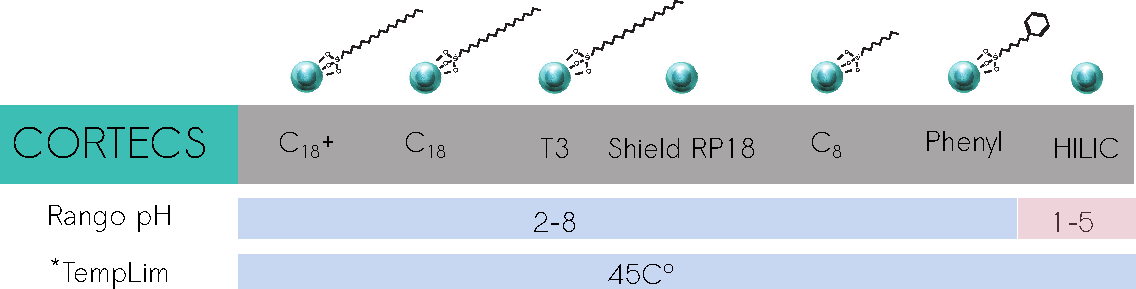
\includegraphics[width=1\linewidth]{img/drawing_4}
                \label{fig:drawing4}
            \end{figure}

        \end{frame}


        \begin{frame}{CORTECS HILIC 2.7$\mu m \quad 3\times 150 mm$}
            \textbf{HILIC:} Hydrophilic-interaction cromatography. Es empleado para separar analitos extremadamente polares.
            \begin{table}
                \centering
                \begin{tabular}{ccc}
                    CORTECS 2.7 $\mu m$ Aplicaciones &Código de búsqueda & Pagina \\
                    \hline
                    Medicamentos (básicos)& WA60707 &49\\
                    en agua de río&  &\\
                    HILIC Control de Calidad & WA64704 & 50 \\
                    Morfina y Metabolitos  & WA64701 & 51 \\
                    \hline
                \end{tabular}
            \end{table}
        \end{frame}

        \begin{frame}{CORTECS Phenyl 2.7$\mu m \quad 3\times 150 mm$}

        \end{frame}


      \subsection{XBRIDGE}

        \begin{frame}{}
            \begin{center}
                \textbf{\LARGE XBridge}
            \end{center}
            \begin{figure}
                \centering
                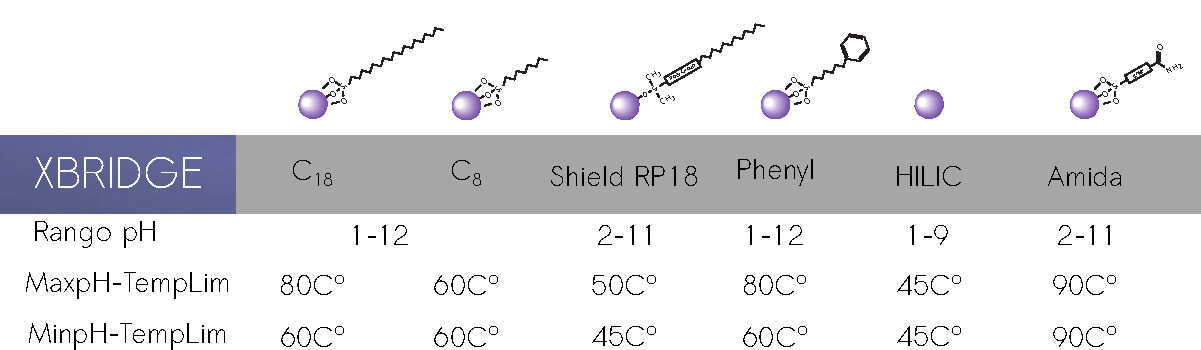
\includegraphics[width=1\linewidth]{img/drawing_5}
                \label{fig:drawing5}
            \end{figure}

        \end{frame}


      \subsection{XSELECT}

      \begin{frame}{}
          \begin{center}
              \textbf{\LARGE XSelect}
          \end{center}
          \begin{figure}
              \centering
              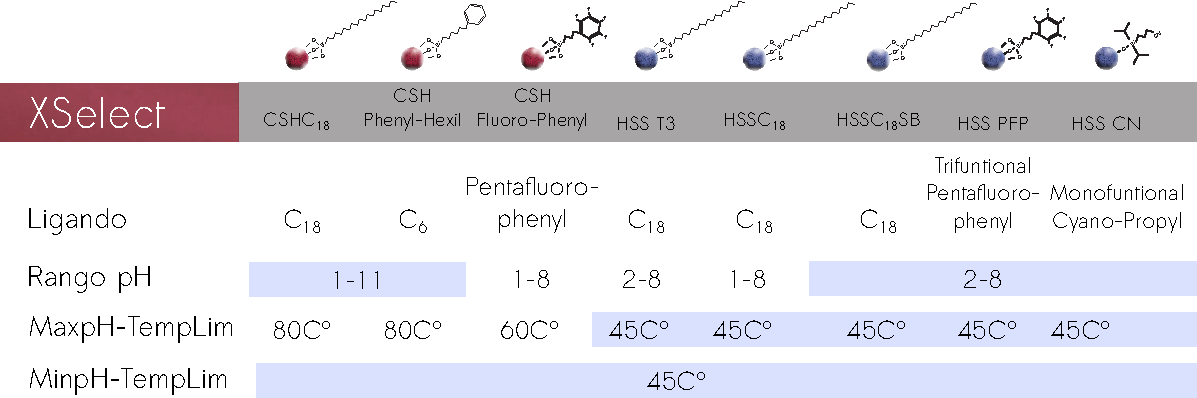
\includegraphics[width=1\linewidth]{img/drawing_6}
              \label{fig:drawing6}
          \end{figure}

      \end{frame}

\end{document}